%%%%%%%%%%%%%%%%%%%%% chapter.tex %%%%%%%%%%%%%%%%%%%%%%%%%%%%%%%%%
%
% esempio di capitolo
%
% Usare questo  file come template per il vostro documento.
%
%%%%%%%%%%%%%%%%%%%%%%%% Springer-Verlag %%%%%%%%%%%%%%%%%%%%%%%%%%

\chapter{Dinamica dei corpi rigidi}
\label{dinamica_corporigido}
\section{Dinamica vincolata}
\subsection{Matrice Jacobiana dei vincoli $C_q$} \label{sec:Jabobian}
\paragraph{Vincoli}
Per bloccare alcuni gradi di libertà di un sistema e permetterne altri vengono inseriti vincoli (\emph{constraints}) nel sistema. A seconda di quanti e quali gradi di libertà vengono bloccati esistono vari tipi di vincoli, uno dei più comuni è la cerniera (\emph{revolute joint}) illustrata in figura \ref{fig:2.1}.
\begin{figure}[ht]
\centering
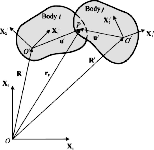
\includegraphics[height=7cm]{revolute.pdf}
\caption{Cerniera tra i corpi i e j}
\label{fig:2.1}
\end{figure}
In questo caso i corpi i e j hanno un solo grado di libertà relativo, ovvero la rotazione (si noti che siamo nel caso di moto piano).
In un sistema multibody le coordinate possono essere messe in relazione grazie ai vincoli, si potrà quindi scegliere quali coordinate sono dipendenti e quali indipendenti. 
Ogni equazione vincolare può eliminare una coordinata (che può essere quindi scritta in funzione di un'altra)
Perciò, un sistema di  $n$ coordinate ed $n_c$ equazioni vincolari ha $n-n_c$ coordinate indipendenti. 
Le coordinate indipendenti sono dette anche Gradi Di Libertà (GDL) del sistema.

\paragraph{Matrice Jacobiana $C_q$} Per poter considerare la presenza dei vincoli nella soluzione sarà necessario trovare relazioni tra i gradi di libertà dovuti ai vincoli, le quali andranno poi organizzate in un sistema di equazioni, per definire infine una matrice dei vincoli $C(q,t)$. \newline Le condizioni imposte da ciascun vincolo danno luogo ad un sistema di equazioni del tipo:
\begin{equation} \label{eq:Cqt}
C(q,t) = 0
\end{equation}
La relazione che definisce una cerniera nel caso di moto piano come mostrato in figura \ref{fig:2.1} ad esempio è data imponendo che la posizione del punto P considerato solidale al corpo i sia uguale alla posizione di P considerato solidale a j:
\[\overline{R}_i + A_i\overline{u}_i -\overline{R}_j - A_j\overline{u}_j = 0\]
Dove con R si indica la posizione assoluta delle origini dei riferimenti solidali ad i e j, con A la matrice di rotazione, con u la posizione di P e con i pedici i e j si indica che l'entità è relativa a quel corpo.
Ogni vincolo dà luogo ad numero di equazioni pari al suo grado di vincolo (ossia il numero di gradi di libertà bloccati dal vincolo). Poiché il sistema dovrà essere risolto numericamente con l'algoritmo di Newton-Raphson si rende necessario derivare rispetto agli spostamenti le equazioni dei vincoli ed organizzare i coefficienti in una matrice. La matrice così ottenuta sarà la matrice Jacobiana dei vincoli o sempicemente Jacobiano:
\begin{equation}
\label{eq:jacobian}
C_q =  \begin{bmatrix}
\frac{\partial C_1}{\partial q_1} & \frac{\partial C_1}{\partial q_2} & \qquad ... \qquad & \frac{\partial C_1}{\partial q_n} \\\
\frac{\partial C_2}{\partial q_1} & \frac{\partial C_2}{\partial q_2} & \qquad ... \qquad & \frac{\partial C_2}{\partial q_n} \\ . \\. \\ 
\frac{\partial C_{n_c}}{\partial q_1} & \frac{\partial C_{n_c}}{\partial q_2} & \qquad ... \qquad & \frac{\partial C_{n_c}}{\partial q_n}
\end{bmatrix} 
\end{equation}
Sviluppando l'equazione \ref{eq:Cqt} si può quindi scrivere:
\begin{equation} \label{jacobian_expansion}
C_q \delta q = 0
\end{equation}
Prendendo ad esempio il sistema con 2 soli corpi in figura [\ref{fig:2.1}] si ottiene:
\[ (C_1 , C_2)^T = \overline{R}_i + A_i\overline{u}_i -\overline{R}_j - A_j\overline{u}_j \]
Il sistema ha 6 coordinate e 2 equazioni vincolari date dall'unica cerniera. Le derivate rispetto alle posizioni sono banali, per quanto riguarda le rotazioni:
\[\frac{\partial C_1}{\partial \theta_i } = \frac{\partial A_i}{\partial \theta_i } \overline{u}_i  = A_i'\overline{u}_i\]
Dove A' indica la derivata della matrice di rotazione rispetto all'angolo che la definisce. Indicando un $u_{i,1}, u_{i,2}, u_{j,1} u_{j,2}$ le componenti nel primo e secondo asse dei vettori $u_i$ ed $u_j$, si può scrivere:
\begin{equation} C_q \delta q = 
\begin{bmatrix}
1 \quad & 0\quad & -u_{i,1}sin\theta_i-u_{i,2}cos\theta_i \quad& -1 \quad& 0 \quad& -u_{j,1}sin\theta_j-u_{j,2}cos\theta_j \\
0 \quad& 1 \quad& u_{i,1}cos\theta_i-u_{i,2}sin\theta_i \quad& 0 \quad& -1 \quad& u_{j,1}cos\theta_j-u_{j,2}sin\theta_j
\end{bmatrix}
\begin{pmatrix}
\delta R_{i,1} \\ \delta R_{i,2} \\ \delta \theta_i \\ \delta R_{j,1} \\ \delta R_{j,2} \\ \delta \theta_j 
\end{pmatrix} = 0
\end{equation}

\subsection{Moltiplicatori Lagrangiani}
Nella sezione  \ref{sec:Jabobian} è stato introdotto il calcolo dello Jacobiano e il concetto di coordinate dipendenti ed indipendenti. Per la soluzione numerica è conveniente considerare le reazioni vincolari come segue. \newline
\paragraph{Singolo Vincolo}
il jacobiano del vincolo $C_q$ tra i corpi \emph{i} e \emph{j} viene spezzato in 2 matrici:
\begin{equation} \label{eq:jacobian_composition}
C_q = \left[ C_{q^i} C_{q^j}\right]
\end{equation}
Si definisce quindi un sistema di forze \emph{equipollente} agente nelle origini dei sistemi di riferimento dei corpi di i e j. $\overline{\lambda}$ è il vettore delle forze e dei momenti esercitati dal vincolo:
\begin{equation} \label{eq:lambda}
\overline{\lambda} = - \begin{bmatrix} \overline{F} \\ \overline{M}
\end{bmatrix} \end{equation}
Le forze di reazione agenti sui corpi i e j sono:
\begin{equation}
\overline{F}^i = -\overline{\lambda} = 
\begin{bmatrix} \overline{F} \\ \overline{M} \end{bmatrix} \qquad ; 
\qquad \overline{F}^J = \overline{\lambda} = -\begin{bmatrix} \overline{F} \\ \overline{M} \end{bmatrix}
\end{equation}
Mentre, considerate nelle origini come sistema equipollente si ottiene:
\begin{equation}
Q^i_c = \begin{bmatrix} \overline{F} \\ \overline{M} + A^i\overline{u}^i_p x F \end{bmatrix} \qquad ; 
\end{equation}
Dove $\overline{u}^i_p$ è il vettore posizione di P (ove è applicato il vincolo) nelle coordinate di i e $A^i$ matrice di rotazione di i.
Da \cite{shabana94} si ha che:
\[A^i\overline{u}^i_p x F = {\overline{u}^i_p}^T {A_\theta^i}^T  \]
Si osserva quindi che le reazioni generalizzate possono essere espresse come:
\begin{equation}
\label{eq:lagrangemulti_to_reaction}
Q_c^i = -C^T_{q^i} \lambda
\end{equation}
\paragraph{Più vincoli}
Si può estendere la procedura illustrata al caso di più corpi collegati da più vincoli. Se sul corpo i ci sono $n_i$ vincoli le equazioni che li descrivono vengono espresse come:
\begin{equation} \label{eq:multiplejointeq} \begin{cases}
C_1(q,t) = 0 \\ C_2(q,t) = 0 \\ . \\ .\\ . \\ C_{n_i}(q,t) = 0
\end{cases}
\end{equation}
Ogni equazione vettoriale in \ref{eq:multiplejointeq} contiene tante equazioni quanti sono i \emph{gradi di vincolo} (gradi di libertà eliminati dal vincolo) del vincolo corrispondente. Dalla \ref{eq:lagrangemulti_to_reaction} si può estendere:
\begin{equation}\begin{cases}
Q_1^i = -\left( C_1 \right)^T_{q^i} \lambda_1 \\ Q_2^i = -\left( C_2 \right)^T_{q^i} \lambda_2 \\ . \\
Q_{ni}^i = -\left( C_{ni} \right)^T_{q^i} \lambda_{ni}
\end{cases} \end{equation}
Indicando con $Q^i_c$ la risultante delle reazioni vincolari sul corpo \emph{i} si può scrivere:
\begin{equation}\label{eq:reactions_result_body}
Q^i_c = -\left[ \left( C_1 \right)^T_{q^i} \quad \left( C_2 \right)^T_{q^i} \qquad \cdot\cdot\cdot 
\qquad \left( C_{ni} \right)^T_{q^i} \right] \begin{bmatrix}
\lambda_1 \\ \lambda2 \\ \cdot \\ \cdot \\ \cdot \\ \lambda_{n_i} 
\end{bmatrix} \end{equation}
Estendendo il calcolo a tutti gli $n_b$ corpi del sistema si calcolano le reazioni generalizzate dell'intero sistema $Q_c$. Essendo:
\[Q_c^i = -C^T_{q^i}\lambda\]
Si otterrà:
\begin{equation} \label{eq:sys_ge_reactions}
Q_c = \left[{Q_c^1}^T \qquad {Q_c^2}^T \quad \cdot \quad \cdot \quad \cdot {Q_c^{n_b}}^T\right]^T = \begin{bmatrix}Q_c^1 = -C^T_{q^1}\lambda \\ Q_c^2 = -C^T_{q^2}\lambda
\\ \cdot \\ \cdot \\ \cdot \\ Q_c^{n_b} = -C^T_{q^{n_b}}\lambda \end{bmatrix}
\end{equation}
Estendendo la composizione dello jacobiano in \ref{eq:jacobian_composition} si può quindi scrivere:
\begin{equation} \label{eq:reactions_result_sys}
Q_c = - \left[ C_{q^1} \qquad C_{q^2} \quad \cdot\quad\cdot\quad\cdot\quad Q_{q^{n_b}} \right]^T \lambda = -C_q^T\lambda
\end{equation}
\section{Equazioni della dinamica vincolata}
Per estendere quanto visto riguardo ai sistemi di particelle  nel cap. \ref{Formula di Lagrange} a sistemi di corpi rigidi sono necessarie alcune considerazioni:
\paragraph{Cinematica del corpo rigido}
La posizione di un corpo si esprime per mezzo di una traslazione dell'origine ed una rotazione:
\begin{equation} \label{eq:body_point_pos}
r^i = R^i + A^i\overline{u}^i
\end{equation}
Dove r è la posizione assoluta del punto P appartenente al corpo i, R è la posizione dell'origine del riferimento solidale ad i, A è la matrice di rotazione del corpo i e $\overline{u}$ è la posizione relativa di P. La velocità si ottiene derivando rispetto al tempo:
\begin{equation} \label{eq:body_point_vel}
\dot{r}^i = \dot{R}^i + \dot{A}^i\overline{u}^i = \dot{R}^i - A^i \tilde{\overline{u}}^i\overline{G}\dot{\theta}^i
\end{equation}
Con $\theta = \overline{q}$ quaternione unitario o vettore dei parametri di Eulero (indifferentemente), ed $\overline{G} = 2F(q^*)_-$ dell'equazione \ref{eq:1.9}. $\tilde{\overline{u}}$ è la matrice emisimmetrica ottenuta dalla posizione relativa $\overline{u}$ del generico punto P:
\begin{eqnarray} \tilde{\overline{u}}  = \begin{bmatrix}
0 & -x_3^i & x_2^i \\ x_3^i & 0 & -x_1^i \\ -x_2^i & x_1^i & 0 \end{bmatrix}\end{eqnarray}
Lo spostamento può essere dunque scritto in forma partizionata:
\begin{equation} \label{eq:body_point_vel_partform}
\dot{r}^i = \left[ I \qquad - A^i\tilde{\overline{u}}^i\overline{G}^i\right] \begin{bmatrix}\dot{R}^i \\ \dot{\theta}^i \end{bmatrix}  \end{equation}
\subsection{Matrice di massa}
Estendendo ad un corpo la definizione di energia cinetica data nell'equazione \ref{eq:part_kinenergy} si ottiene:
\begin{align} \label{eq:body_kinenergy}
T^i &= \frac{1}{2}\int_{V^i}\rho^i\dot{r}^{i^T} \dot{r}^idV^i 
\\ &= \frac{1}{2}\int_{V^i}\rho^i [\dot{R}^{i^T}\quad \dot{\theta}^{i^T}] \begin{bmatrix}I \\ - \overline{G}^{i^T}\tilde{\overline{u}^{i^T}A^{i^T}} \end{bmatrix} [I \quad -A^i\tilde{\overline{u}}^i\overline{G}^i] \begin{bmatrix} \dot{R}^i \\ \dot{\theta}^i \end{bmatrix}  dV^i \nonumber \\ &= \frac{1}{2}[\dot{R}^{i^T}\quad \dot{\theta}^{i^T}]\left\{\int_{V^i}\rho^i \begin{bmatrix}
I & -A^i\tilde{\overline{u}}^i\overline{G}^i \\ \quad sym_b \quad & \overline{G}^{i^T}\tilde{\overline{u}}^{i^T}\tilde{\overline{u}}^i\overline{G}^i
\end{bmatrix}  dV^i\right\} \begin{bmatrix} \dot{R}^i \\ \dot{\theta}^i \end{bmatrix} \nonumber
\\ &= \frac{1}{2}\dot{q}_r^{i^T}M^i\dot{q}_r^i
\end{align}
Con $sym_b$ si intende che il blocco è simmetrico.
$M^i$ è la \emph{matrice di massa} del corpo rigido i di volume $V^i$:
\begin{align}
M^i &= \int_{V^i}\rho^i \begin{bmatrix}
I & -A^i\tilde{\overline{u}}^i\overline{G}^i \\ \quad sym_b \quad & \overline{G}^{i^T}\tilde{\overline{u}}^{i^T}\tilde{\overline{u}}^i\overline{G}^i \end{bmatrix}  dV^i \\
&= \begin{bmatrix} m^i_{RR} & m^i_{R\theta} \\ \quad sym_b\quad &m^i_{\theta\theta}  \end{bmatrix} \end{align}
Si verifica facilmente che $M^i_{RR} = m^iI^{3x3}$ con $m_i$ massa dell'i-esimo corpo.
La matrice $M_{RR}$ associata alla traslazione del corpo è quindi una matrice diagonale costante.
La matrice associata all'interazione di rotazione e traslazione $m_{R\theta}$, ricordando che $a^i$ e $\overline{G}^i$ non dipendono dallo spazio si può esprimere come:
\begin{equation}
m^i_{R\theta} = - \int_{V^i}\rho^iA^i\tilde{\overline{u}}^i\overline{G}^idV^*i = -A^i \left[ \int_{V^i}\rho^i\tilde{\overline{u}}^i dV^i \right]  \overline{G}^i = -A^i\tilde{\overline{U}}^i\overline{G}^i
\end{equation}
Si noti che, qualora l'origine del riferimento coincida con il baricentro del corpo, $\tilde{\overline{U}}^i$ si annulla per la definizione di baricentro. 
Procedendo similmente per $m^i_{\theta\theta}$ si ottiene: \begin{align}
m^i_{\theta\theta} &= \overline{G}^{i^T}I_{\theta\theta}\overline{G}^i \\
I_{\theta\theta} &= \int_{V^i} \rho^i\tilde{\overline{u}}^{i^T} \tilde{\overline{u}}^i dV^i \\
I_{\theta\theta}&= \begin{bmatrix}i_{11} & i_{12} & i_{13} \\ \quad & i_{22} & i_{23} \\ sym & \quad & i_{33}\end{bmatrix}
\end{align}
Con $sym$ si nitende che la matrice è simmetrica
Con \begin{align} \label{eq:inertia_moment}
i_{jj} &= \int_{V^i} \rho^i[(x_k^i)^2+(x_l^i)^2]dV^i \qquad j\neq k\neq l\neq j ; \quad j,k,l = 1,2,3 \\
\label{eq:inertia_prod} i_{jk} &= \int_{V^i} \rho^ix_j^ix_k^i dV^i \qquad \qquad\qquad j\neq k \qquad j,k = 1,2,3
\end{align}
Gli elementi diagonali della matrice $I_{\theta\theta}$ descritti nell'equazione \ref{eq:inertia_moment} sono detti momenti d'inerzia, mentre i termini non diagonali di \ref{eq:inertia_prod} sono chiamati prodotti d'inerzia. Questi ultimi si annullano qualora il riferimento solidale al corpo sia \emph{principale di inerzia}.
L'energia cinetica di un corpo rigido può essere così scomposta:
\begin{align} \nonumber
T^i_{RR} &= \frac{1}{2}\dot{R}^{i^T}m^i_{RR}\dot{R}^i; \qquad T^i_{r\theta} = \dot{R}^{i^T}m^i_{r\theta}\dot{\theta}^i, \\ \nonumber
T^i_{\theta\theta} &= \frac{1}{2}\dot{\theta}^{i^T}m^i_{\theta\theta}\dot{\theta}^i =  \frac{1}{2} \overline{\omega}^{i^T}\overline{I}^i_{\theta\theta}\overline{\omega}^i
\end{align}
\subsection{Equazioni della dinamica dei corpi rigidi vincolati}
\paragraph{Equazioni della Dinamica}
L'equazione di Lagrange \ref{eq:lagrange_matrix} per i corpi rigidi assume la forma:
\begin{align} \label{eq:lagrange_body} \nonumber
\frac{d}{dt}\left( \frac{\partial T^i}{\partial\dot{q}}\right) -\frac{\partial T^i}{\partial q} -Q^i_e = 0 \\ \nonumber
\frac{d}{dt}\frac{\partial}{\partial \dot{q}}\left( \frac{1}{2}\dot{q}^{i^T}M^i\dot{q}^i \right) -\frac{\partial T^i}{\partial q} -Q^i_e = 0 \\ \nonumber
\frac{d}{dt}\left( M^i\dot{q}^i \right) -\frac{\partial T^i}{\partial q} -Q^i_e = 0 \\ 
 M^i\ddot{q}^i +\dot{M}^i\dot{q}^i -\frac{\partial T^i}{\partial q} -Q^i_e = 0 
\end{align}
Si consideri:
\begin{equation} \label{eq:Qv}
Q_v^i = -\dot{M}^i\dot{q}^i+\frac{\partial T}{\partial q}
\end{equation}
In verità l'espressione si riduce a \cite{shabana2005} : % pag 149 PDF 
\begin{align} \nonumber
Q_v^i = -\dot{M}^i\dot{q}^i+\left(\frac{\partial T}{\partial q}\right)^T =  [0_3^T \qquad -2\overline{\omega}^{i^T} \overline{I}^i_{\theta\theta}\dot{\overline{G}}^i ]
\end{align}
Infine, osservando che le equazioni sopra valgono per ogni corpo \emph{i} si ottiene in forma matriciale:
\begin{equation} \label{eq:dyn_sys_1stline}
M\ddot{q}+C_q^T\lambda = Q_e + Q_v
\end{equation}
con: 
\[M = \begin{bmatrix}
M^1 & \quad & \quad & \quad \\ \quad & M^2 & \quad & 0 \\ 0 & \quad & \ddots & \quad \\ \quad & \quad & \quad & M^{n_b}\end{bmatrix}\]
\[C_q^T = \begin{bmatrix} C^T_{q^1} \\ C^T_{q^2} \\ \vdots \\ C^T_{q^{n_b}} \end{bmatrix}; \qquad
Q_e = \begin{bmatrix} Q_e^1 \\\ Q_e^2 \\ \vdots \\ Q_e^{n_b} \end{bmatrix}; \qquad
Q_v = \begin{bmatrix} Q_v^1 \\\ Q_v^2 \\ \vdots \\ Q_v^{n_b} \end{bmatrix} \]
\textit{Si noti l'aggiunta di un termine vincolare e l'utilizzo del caso con coordinate indipendenti. Si veda il paragrafo seguente per approfondimenti.} \newline
Per considerare le equazioni di vincolo si deriva 2 volte rispetto al tempo l'equazione \ref{eq:Cqt} ottenendo:
\[C_q\ddot{q} + C_{tt} + (C_q\dot{q})_q\dot{q} + C_{qt}\dot{q}\]
Dove i pedici \emph{t} e \emph{q} indicano la derivazione parziale rispetto a tempo e posizione.
Considerando:
\begin{equation} \label{eq:Qd}
Q_d = - C_{tt} - (C_q\dot{q})_q\dot{q} - C_{qt}\dot{q}
\end{equation}
Da cui;
\begin{equation} \label{eq:dyn_sys_2ndline}
C_q\ddot{q} = Q_d
\end{equation}
Le equazioni \ref{eq:dyn_sys_1stline} e \ref{eq:dyn_sys_2ndline} danno luogo al seguente sistema:
\begin{equation} \label{eq:dyn_sys}
\begin{bmatrix} M & C_q^T \\ C_q & 0 \end{bmatrix}
\begin{bmatrix} \ddot{q}\\ \lambda \end{bmatrix} = 
\begin{bmatrix}
Q_e + Q_v \\ Q_d
\end{bmatrix}
\end{equation}
Questo sistema lineare può essere risolto per il vettore delle accelerazioni $\ddot{q}$ e dei moltiplicatori lagrangiani $\lambda$. A partire dalle condizioni iniziali è possibile integrare numericamente le accelerazioni per ottenere velocità e posizioni.
\paragraph{Formulazione Aumentata}
\textbf{Nota:} nella trattazione che porta all'equazione \ref{eq:dyn_sys_1stline} si è eliminato il termine $\delta q$ considerando le coordinate indipendenti. Nel caso di sistema vincolato tuttavia alcuni gradi di libertà saranno dipendenti a causa della presenza dei vincoli. La \emph{formulazione aumentata} \cite{shabana94} permette di trattare indipendentemente le coordinate di sistemi vincolati. \newline
Si considerino le equazioni \ref{eq:lagrange_body} e \ref{jacobian_expansion} ($Q_v$ si consideri compreso nel termine $Q_e$):
\begin{align} \nonumber \ \delta q^T\left[ M\ddot{q} - Q_e \right] = 0 \\ \nonumber
C_q \delta q = 0
\end{align}
Si deduce che  \[ \lambda^T C_q \delta q = 0 \] e quindi 
\[\delta q^T\left[ M\ddot{q} - Q_e +C_q^T\lambda \right] = 0 \]
Il vettore delle posizioni q viene partizionato in coordinate dipendenti ed indipendenti, e si ottiene:
\begin{equation}  [\delta q_i^T \quad \delta q_d^T] \left\{ \begin{bmatrix} M_{ii} & M_{id} \\ M_{di} & M_{dd}\end{bmatrix}
\begin{bmatrix}\ddot{q}_i \\ \ddot{q}_d \end{bmatrix}
- \begin{bmatrix} Q_{ei} \\ Q_{ed} \end{bmatrix}+ \begin{bmatrix}
C_{qi}^T \\ C_{qd}^T\end{bmatrix} \lambda
\right\}   = 0 \end{equation}
Ne consegue che:
\begin{align} \label{eq_aug_for_a}
\delta q_i^T \left[ M_{ii}\ddot{q}_i + M_{id}\ddot{q}_d - Q_{e_i} + C^T_{q_i}\lambda \right] = 0
\\ \label{eq_aug_for_b}
\delta q_d^T \left[ M_{di}\ddot{q}_i + M_{dd}\ddot{q}_d - Q_{e_d} + C^T_{q_d}\lambda \right] = 0
\end{align}
Le coordinate dipendenti possono sempre essere scelte in modo che $C_q$ sia non singolare in quanto le equazioni di vincolo sono linearmente indipendenti. Il vettore dei moltiplicatori lagrangiani sarà quindi la soluzione (unica) del sistema di equazioni \begin{equation}
C^T_{q_d} \lambda = Q_{e_d} - M_{id}\ddot{q}_i - M_{dd}\ddot{q}_d
\end{equation}
Ragion per cui i coefficienti di $\delta q$ nell' equazione \ref{eq_aug_for_b} sono tutti uguali a 0. Nell'equazione \ref{eq_aug_for_a} invece, poiché i $q_i$ sono indipendenti: \begin{equation}
M_{ii} \ddot{q}_i + M_{id}\ddot{q}_d +C^T_{q_i} \lambda = Q_{e_i}
\end{equation}
Combinando le 2 equazioni sopra si ottiene:
\[ \begin{bmatrix}  M_{ii} & M_{id} \\ M_{di} & M_{dd} \end{bmatrix}
\begin{bmatrix}\ddot{q}_i \\ \ddot{q}_d \end{bmatrix} +
\begin{bmatrix} C_{qi}^T \\ C_{qd}^T\end{bmatrix} \lambda = 
\begin{bmatrix} Q_{ei} \\ Q_{ed} \end{bmatrix}
\]
Da cui la forma generale: \begin{equation}
M\ddot{q} + C^T_q = Q_e	\end{equation}
Dando per noto il vettore delle forze esterne $Q_e$, le incognite sono $\ddot{q}$ e $\lambda$. Il numero di incognite è pari al numero di gradi di libertà indipendenti \emph{n} più il totale dei gradi di vincolo $n_c$. per questo viene aggiunta l'equazione \ref{eq:dyn_sys_2ndline}.